\section{Background}

\begin{frame}{Background}

%\setbeamercovered{transparent=50}
%\setbeamercovered{transparent}

\begin{itemize*}
\item Demand from both industry and academy on accurate modelling of
  electrokinetic systems.
\item Example of applications: drugs, biological chips, fuel cells...
\item A lattice-Boltzmann code is developed at Chalmers to deal with
  transport through complicated structures.
\item This work aims to investigate how electric effects may be integrated.
\end{itemize*}


\end{frame}

\begin{frame}[plain]
\begin{figure}
\begin{center}
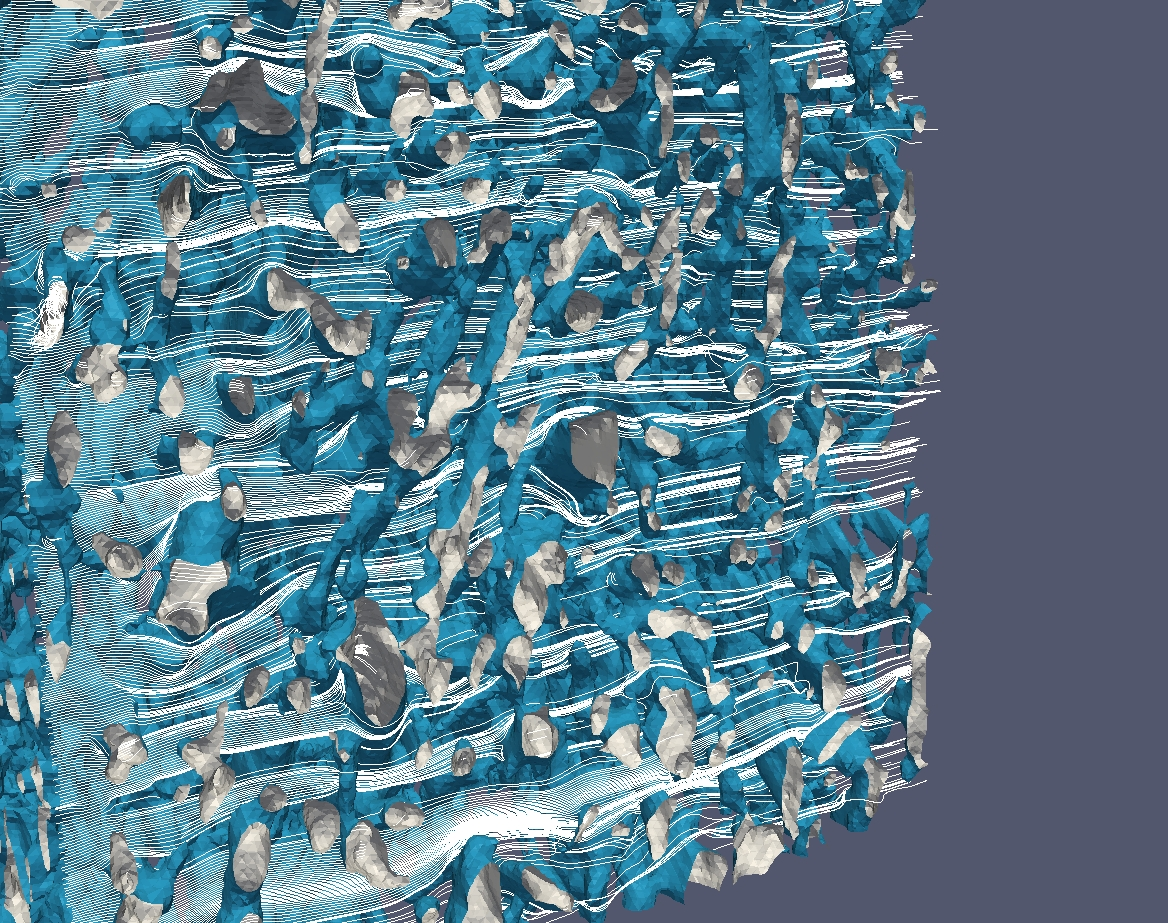
\includegraphics[width=1.0\textwidth]{fig/diffusion_w4.jpg}
\end{center}
%\caption{Visualisation of the coupling between the three equations
%  present in the model. Poisson's equation (PE), The set of
%  Nernst-Planck equations (NP$_1$ ... NP$_n$) for the different ion
%  species and the Navier-Stokes equations (NS). The dependencies have
%  also be marked with arrows indicating what quantities for a certain
%  equation that are needed from an other.}
%\label{fig:coupling}
\end{figure}
\end{frame}
